\documentclass{report}

\usepackage[utf8]{inputenc}
\usepackage[margin=1.0in]{geometry}

\usepackage{amsmath}        % math

\usepackage{graphicx}

\usepackage{fancyhdr}       % The package
\pagestyle{fancy}           % Enforce fancy settings
\fancyhf{}                  % Null all other options
\fancyhead[R]{Page \thepage}

% Macros
\newcommand{\npar}{\par\noindent}
\newcommand{\vpar}{\vspace{1em}\npar}
\newcommand{\nnote}{\npar \S \textbf{ Note: }}
\newcommand{\note}{\vpar \S \textbf{ Note: }}

\usepackage{tgpagella}      % Set the font
\begin{document}
\tableofcontents{}

\chapter{Cloud Computing Basics}

\textbf{Cloud computing} is the practice of using remote servers to process and store data, instead of a local server or personal machine. With that being said, enjoy!

\section{Servers and Clients}

\par A \textbf{server} is a computer/software that processes requests, that is, receives data from a client or another server and delivers data based on those requests. A \textbf{client} is a computer/software that accesses a service made available by a server.

\section{Server Hardware and Cloud Servers}

\par Server hardware runs the server (duh), which is expected to have no downtime. The standard practice for enterprise companies is to have data centers with air-conditioned server racks full of computers, which also provide as backups for all possible contingencies. For a poor individual however, the best solution is to throw a dedicated computer with a network cable in a closet.

\note The unit of measure for the height of one rack frame is a rack unit (U), and a typical server rack is 42U tall.

\vpar The alternative is the \textbf{cloud computing model}, where server hardware is rented out from a large service provider. The provider purchases their own hardware, builds/maintains the data center, and handles the networking. There are various financial models for users purchasing server resources: pay-as-you-go (charging based on actual consumption), pure subscription to a set amount of resources, etc.

\vpar The main advantage of the cloud computing model is that it allows companies to save on operating expenses (opex), and not focus on hiring IT professionals or managing hardware.

\section{Public vs. Private Cloud}

\par The \textbf{public cloud} is the cloud computing model where the service provider handles all of the maintenance of the server hardware -- none of it is owned by the user purchasing server space. The resources are usually given on shared hardware, but the good news is that the buyer doesn't have to worry about any of the finer details. This model is the one most people understand about cloud computing.

\vpar The \textbf{private cloud} is where services are provided and deployed on private infrastructure, that is, the company manages the hardware themselves. The advantage of this model is that the company gets control of the environment and management of cloud resources. This model is less the cloud computing model described above and more just the company owning their own server hardware (literally).

\newpage
\section{Infrastructure as a Service (IaaS)}

\subsection{About}

\par \textbf{Infrastructure as a Service} is the cloud computing model as we know it -- the computing resources are given by the provider, and the buyer has self-service to the given resources (monitoring computers, changing networking, storage). Some popular examples are Google Cloud, Amazon AWS, and Microsoft Azure.

\subsection{Difference between On-Premises, Iaas, PaaS, SaaS}

\par A quick overview of the other different service offerings:
\begin{itemize}
    \item On-Premises sounds exactly like what it's supposed to be: the computers and software are installed on the premise of the organization using the software.
    \item With Platform as a Service, users are mainly concerned with development and deployment of their application, as the server, storage, and networking is covered by the provider. Two common examples are Heroku and Amazon Elastic Beanstalk.
    \item With Software as a Service, users don't have to do anything but use the software provided. The creator of the software (the seller) has to maintain the application and the server running it. The most well-known examples are Google Apps, Dropbox, and Salesforce.
\end{itemize}

\npar Below is a diagram that illustrates the various control levels of the different types of offerings (provided by \verb|bmc.com|):
\begin{center}
    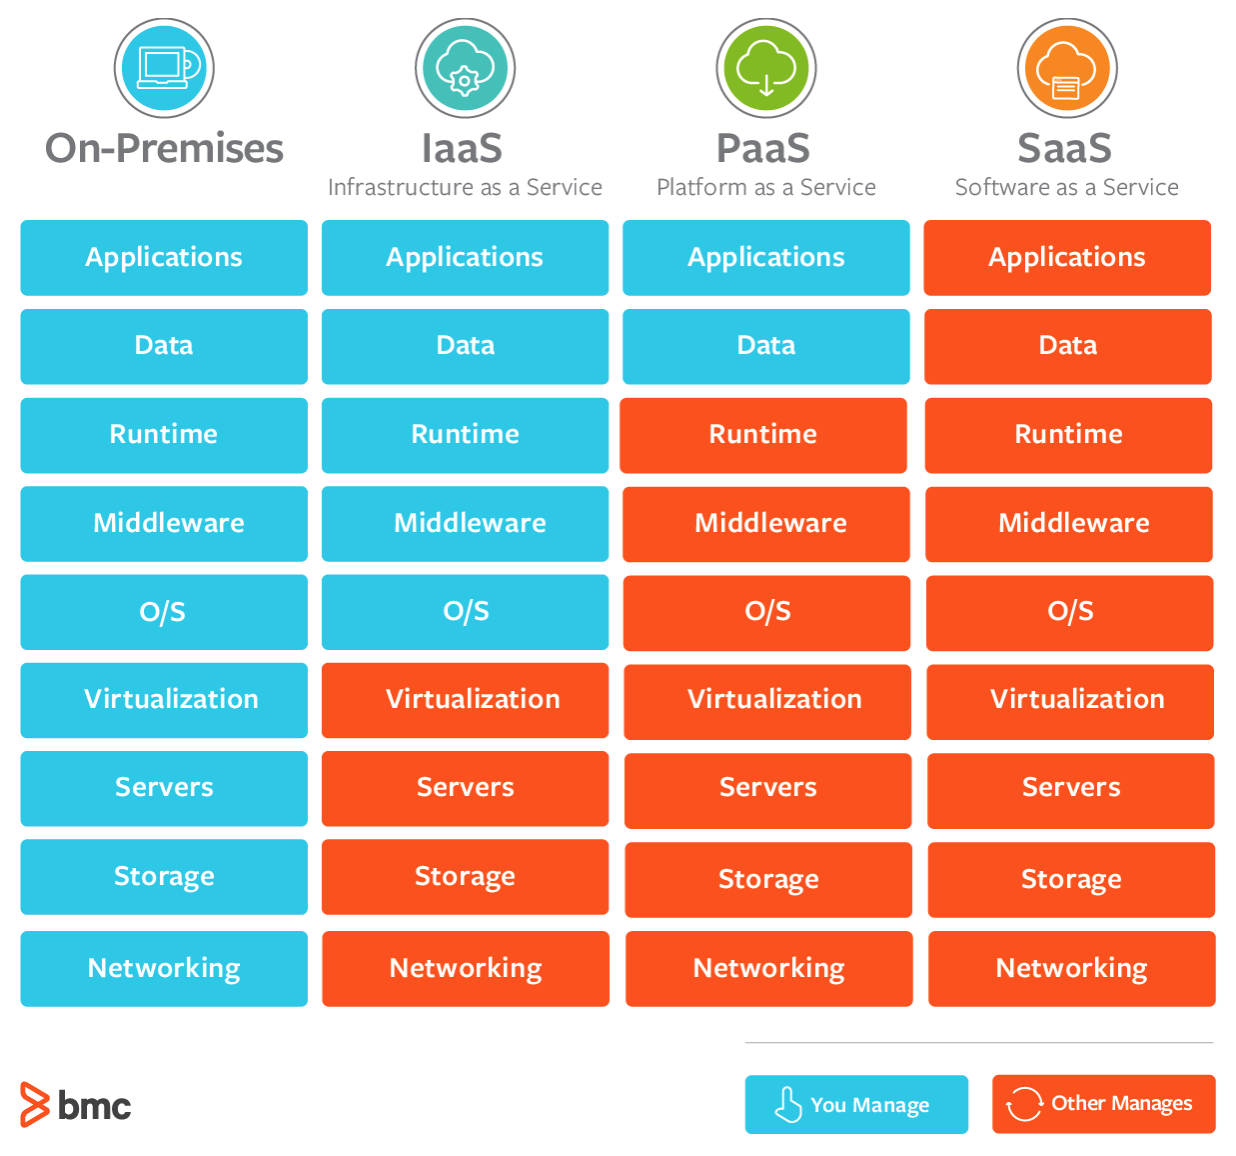
\includegraphics[scale=0.65]{1-4-2.png}
\end{center}

%
% WORK IN PROGRESS
%
\section{Cloud Resource Management}

\subsection{Security Groups}

\par Security groups are a way of filtering the traffic that comes in and out of a cloud instance. Typically, a security group will allow you to specify what protocol, port range, source, and direction (inbound/outbound) packets can pass through. Packets which don't match a rule will be dropped.

\chapter{Networking}

\section{IP Addresses}
\par Internet Protocol (IP) addresses are used to identify devices in a network (both local and wide).

\subsection{IPv4}
\par An IPv4 (the 4th version of IP) address consists of 4 bytes (32 bits), delimited by a period/dot. Specifically, an IPv4 address is of the form \verb|xxxxxxxx.xxxxxxxx.xxxxxxxx.xxxxxxxx| or is translated into some decimal form like \verb|192.168.0.1|.

\note Subnetting, or netmasking, is a technique to divide a network for performance/management. A \textbf{subnet mask} is a bitmask which will provide the network address when a logical AND is applied to the IP address. A subnet mask is written the same way as an IP address -- its shorthand, represented as \verb|/xx| and appended to the end of an IP, shows how many of the first \verb|xx| bits of the mask are 1s. For example, with the IP address \verb|192.168.0.1/24|, the 24 means the first 24 bits of the subnet mask are ones, which can be written as \verb|255.255.255.0|.

\vpar IPv4 address are split into 5 distinct classes:
\begin{itemize}
    \item A: The first byte value ranges from 0 to 127 with a subnet mask of 8 (first byte for network address, remaining three for host addresses).
    \item B: The first byte value ranges from 128 to 191 with a subnet mask of 16 (first two bytes for network address, remaining two for host addresses).
    \item C: The first byte value ranges from 192 to 223 with a subnet mask of 24 (first three bytes for network address, remaining one for host addresses).
    \item D: The first byte value ranges from 224 to 239, which is used for multicast addresses (whose packets then get distributed to multiple recipients, per the name).
    \item E: The first byte value ranges from 240 to 255, and these IPs are used for experimental purposes.
\end{itemize}

\npar One of the main issues with IPv4 is that its range of addresses have all been used (~4 billion addresses, in Sep. 2015), and that broadcasting (sending packets to all clients on the LAN) clogs the network. The solutions to the problems listed are the introduction of IPv6 and NAT, and a router (respectively).

\newpage
\subsection{IPv6}
\par IPv6 is the latest iteration of IP, which is 128 bits long. Other than a wider range of addresses, its benefits include:
\begin{itemize}
    \item Authentication and access control
    \item Smaller header fields (half the size)
    \item 64-bit alignment (faster processing)
    \item Scalable and efficient routing
\end{itemize}

\section{Network Address Translation (NAT)}

\par \textbf{Network Address Translation} (NAT) is one of the other techniques used to circumvent the lack of addresses in IPv4, as well as provide security to local networks. NAT uses private address ranges, where a NAT device (e.g., router) maps a single IP address to the entire private network. The devices in the private network are then given a private IP, and attempts to directly connect to a device using a private IP from a device outside the network will be dropped.

\begin{center}
    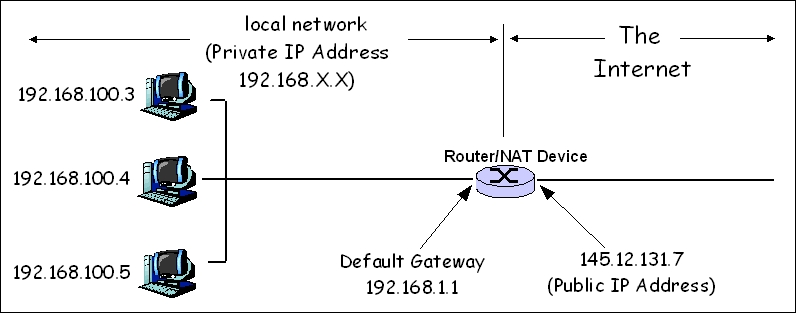
\includegraphics[scale=0.5]{2-2-2-A.jpg}
    \par Example of a NAT (Source: \verb|wikipedia|)
\end{center}

\nnote SNAT = Source NAT, DNAT = Destination NAT: two things the gateway is in charge of handling

\note 192.168.x.x is the typical private network for homes

\section{Domain Name System}

\par \textbf{Domain Name System}, or DNS, is the phonebook of the internet. It takes a domain name and translates it into an IP so browsers can load internet resources.

\section{Floating IP}

\par A \textbf{floating IP} is a public, routable IP address that is obtained from a pool of IPs that a system administrator or cloud provider configures and provides as a server resource.

\chapter{Web Development}

\section{Overview}

\par When a browser (the client) makes a request for a webpage, the workflow looks like this:
\begin{enumerate}
    \item The client makes an async request to the server via HTTP, which looks like this: \verb|GET / HTTP/1.1|
    \item The server receives the request and finds the corresponding HTML file based on given parameters.
    \item The client receives the HTML file, and as the HTML is read, it makes subsequent requests to the server (or an external one) for additional needed files like CSS or JS files. While the requests are being made (or are complete), the browser is rendering the page.
\end{enumerate}

\section{History}

\par Originally, websites were not dynamic -- maps were used for hyperlinking images, table design was popular, and responsive design did not exist (adjusting viewport and display by device).

\vpar Now, all the cool and modern websites have a multitude of CSS libraries (Bootstrap, Material) as well as templating libraries/frameworks (React, Vue) which can generate dynamic content from templates.

\section{HTTP}

\subsection{About}

\par Hypertext Transfer Protocol (HTTP) is the main protocol for the Worldwide Web (WWW), and is created to be human-readable format between the client and server (is also very inefficient). It supports a variety of methods, most commonly GET and POST (for receiving and sending data). HTTP requests come with a variety of request/response headers, which can be viewed in the browser's Developer Tools (in the Network tab).

\newpage
\subsection{URLs}

\par A \textbf{uniform resource locator} (also called a web address) is a reference to a web resource that specifies its location on a network and the mechanism for retrieving it. A sample URL is shown below:

\vpar \verb|https://www.facebook.com:443/users.html?user=ferdman&date=2019#bio|
\vpar Each piece can be categorized:
\begin{enumerate}
    \item \verb|https://| \textbf{Schema}: the protocol being used
    \item \verb|www.facebook.com| \textbf{Server Address}
    \item \verb|:443| \textbf{Port}: defaulted to 80 for http, and 443 for https
    \item \verb|/users.html| \textbf{Path}: doesn't have to include the \verb|.html|, \verb|index.html| of the given path will be defaulted
    \item \verb|?user=ferdman?date=2019| \textbf{Query String}: parameters for the server, which start with \verb|?| and is of the format \verb|k=v|, delimited by \verb|?|
    \item \verb|#bio| \textbf{Anchor}: doesn't get sent to the server, is handled by the browser for navigation (typically)
\end{enumerate}

\nnote Non-printable characters in the query string are encoded, e.g., space = \verb|%20|

\vpar URLs are technically a subset of URIs, because they are more specific locators (URL) for a generic identifier (URI).

\subsection{HTTP Response Codes}

\par For every HTTP response sent back from the server, a three digit number usually comes with it to indicate the status of the response:

\begin{itemize}
    \item 1xx Informational (Continue, Processing, ...)
    \item 2xx Success (OK, Created, ...)
    \item 3xx Redirection (Page Moved, Redirect, ...)
    \item 4xx Client Error (Bad Request, Unauthorized, ...)
    \item 5xx Server Error (Service Unavailable, HTTP Version not supported, ...)
\end{itemize}

\npar The most common codes are 200 (OK), and 404 (Not Found).

\section{XHR, Fetch, and AJAX}

\par XMLHttpRequest, or \textbf{XHR}, is a browser object that allows HTTP requests to be made in JavaScript. Despite its name, it support many datatypes (JSON, SOAP).

\vpar \textbf{Fetch} is a new browser method for sending network requests. Fetch code is much more concise, and supports new functionality (although it lacks some of XHR's capabilities).

\vpar Asynchronous JavaScript and XML, or \textbf{AJAX}, is a general technique for sending asynchronous JavaScript requests. Both XHR and Fetch can be used to achieve this.

\section{REST}

\par \textbf{REpresentational State Transfer}, or REST, is a design pattern for APIs. In essences, a server with a RESTful API will send to the client a \textit{representation of the state} of the requested resource. For example, if we wanted to fetch a specific user (e.g., Ferdman), the API will return the state of the user, including their name, number of posts, friends, etc.

\vpar The need for a RESTful API arised when traditional webpages had servers send back snippets of HTML to render, but the client had no control over the actual handling of the data.

\section{Message Formats}

\par \textbf{JavaScript Object Notation}, or JSON, is the most well-known format. Use it. The main advantages is its readability, as well as its well defined structure and native support in JavaScript.

\vpar Older formats include XML and SOAP, which were different standards of representing data. Both formats failed to see widespread success, and WSDL, an extension of SOAP was created. It allowed users to see what function calls were being made, and it contributed to the now rising SOAP, which sees a lot of use in industry.

\section{Comet and Websockets}

\par Comet is a shitty model for HTTP client/server connections -- it is unidirectional, where the server sends the client data. The main issue with comet is that the client has to repeatedly open new connections with the server to send it more information. The upside is that the server only needs to maintain one connection to send information, which is less expensive.

\vpar In comes \textbf{websockets}, where a two-way connection is maintained between client and server. This is a persistent, low latency connection which removes the problem of long-polling (keeping HTTP connection alive until server has data, which had the overhead of HTTP).

\section{Cookies, Web Sessions, and JWT}

\par \textbf{Cookies} are a small piece of data sent from the server to the client, used to record client state, which is accessed by the web server/client computer for various reasons (authentication, metrics, stalking).

\vpar Cookies are sent through requests by setting the SET-COOKIE header, and one of its main uses is to send stateful information, which avoids leaking information in the query string. Modern implementations of cookie in a client/server setting will involve signing the information in the cookie to prevent tampering.

\vpar However, as the traditional use of cookies aren't completely secure, \textbf{sessions} are a model where the server sends a key which is stored in a cookie. That key is related to some data which is associated server-side.

\vpar JWT, which was not covered in class (feel free to skip), is a web standard for encoding a JSON payload alongside a secret. It works almost like a session ID, but encoded and also has other info.

\section{Speeding Up Requests}

\par Successive HTML requests cause slow loading. How can we speed it up?

\subsection{Caching}

\par We can store content from previous HTTP requests, so that we don't have to make requests for resources we already have. Stored content will have expirations and can be replaced if the content is updated before expiration.

\subsection{Pipelining}

\par Just send a bunch of requests in a pipelined manner.

\subsection{Content Delivery Network (CDN)}

\par A CDN is a system of distributed servers which deliver content to a user based on their geographic location. This technique reduces latency as much as possible; the CDN is responsible for hosting your files on all their machines to deliver your resources quickly.

\section{Proxies}

\par A HTTP proxy is a middleman which routes client requests from a browser to the Internet, while potentially providing features like caching and security. It is usually implemented in the application layer.

\chapter{Databases}

\section{Overview}

\par A database is a piece of software designed to store data reliably and consistently. We do not want to expose the database (duh), which means we should never open up a port to the public -- hackers will scan ports like 3306 (MySQL default) to dig out data.

\section{SQL and Related Syntax}

\par A database is considered a SQL database if the data is defined by schemas and retrieved using Structured Query Language (SQL). The main advantages of using SQL is that you get referential integrity, structured data, and data guarantee.

\vpar Useful components of SQL (ordered by relevance):

\begin{itemize}
    \item DML/CRUD: INSERT, SELECT, UPDATE, DELETE
    \item Data-definition Language (DDL): CREATE, ALTER, DROP
    \item Data-control language (DCL): GRANT, REVOKE for permissioning
\end{itemize}

\subsection{MySQL}

\par Used to be incredibly fast (thus popular), then it got caught up in a bunch of features (triggers).

\section{NoSQL}

\par A \textbf{NoSQL} database is schemaless: for the most part, we can describe these databases as a key-value store. The advantage of this is that adding new "columns" is supposedly faster, since all that has to be done is add more properties to a given object (thus tables aren't locked during column updates). Which means developers can release new software with just some property changes.

\vpar Some "variants" (buzzwords) of NoSQL databases include:

\begin{itemize}
    \item Document systems: databases made to store larger data, such as a pdf scan (not just a JSON string).
    \item Column system: for any given key, you have a set of "columns".
\end{itemize}

\vpar And basically the only use case is if you don't care about your data (jk, if your columns are constantly being changed, this is good too).

\chapter{Virtualization}

\par Virtualization is the act of virtualizing computer hardware and operating system by creating a virtual machine. A virtual machine uses the same underlying hardware resources as the host machine, and a single host machine can host multiple virtual machines.

\vpar A hypervisor is a piece of software that runs virtual machines. It exposes a virtual operating platform for guest machines that has hardware abstractions and any other abstractions that operating systems require to run.

\section{History}

\par Fundamentally emulators are just software that runs instructions, it was initially super slow because emulating commands (say Assembly commands like ADD/SUB) required the overhead of doing \verb|x| with the registers. This initially meant it would take too many commands to run just one -- and that added up. There would be long switch statements to figure out which command to run (same thing -- still ADD, JMP, ...).

\vpar There were two major developments that sped up emulation:

\begin{enumerate}
    \item \textbf{Hypervisor}: Type 1 hypervisors (bare metal), run directly on the hardware and makes it possible to use more of the system resources (run commands on physical hardware). The problem is that emulators are still filled with switch statements...
    \item \textbf{Xen}: A type 1 hypervisor that supports concurrent execution on computer hardware through virtualization (virtual disk, etc). The better way to think about it is that Xen is a adapter for hardware. Later, Intel/AMD added more hardware support, adding control structures (VMCS) which defined the virtual machines and added support for \verb|vmenter| and \verb|vmexit| commands, when the machine needed help from the hypervisor.
\end{enumerate}

\npar Most VMs are run this way now, and we can't even tell it's slow.

\section{Cloud Provider Instances}

\par When creating an instance on a cloud, cloud providers offer a \textbf{flavor} selection, which is a combination of the CPU, memory and disk space of an instance. Additional network options can be configured, such as latency, bandwidth and aggregate transfer.

\newpage
\section{Definitions}

\par Some useful definitions for this section -- measurement unit in parenthesis:
\begin{itemize}
    \item \textbf{Instance}: a virtual machine (VM) running on a server
    \item \textbf{Image}: system/software preinstalled into instance
    \item \textbf{Latency} (ms): amount of time it takes to transfer data. Limited by distance (solvable with a CDN).
    \item \textbf{Bandwidth} (GB/s): amount of data that can be transferred per unit of time
    \item \textbf{Aggregate Transfer} (GB): total amount of data transferred
    \item \textbf{Input/Output Operations per Second} (\textbf{IOPS}) (k (thousands)): it's in the name
\end{itemize}

\section{Disk}

\par Your given storage mechanism -- here we care about:

\begin{itemize}
    \item Latency
    \item Bandwidth
    \item IOPS
\end{itemize}

\npar An average benchmark for some types of disks:

\begin{center}
    \begin{tabular}{ c | c | c | c }
                & Range             & SSD       & HDD \\ \hline
    Latency     & 1 to 20ms         & 1ms       & 10ms \\ 
    Bandwidth   & 100 to 1000MB/s   & 1GB/s     & 100MB/s \\  
    IOPs        & 200k              & 200k      & 20k \\
    Capacity    & 4 to 12000GB      & 1TB       & 12TB \\
    Capacity/\$ &                   & 10GB/\$   & 33GB/\$\\
    \end{tabular}
\end{center}

\section{Networking}

\par Your given internet connection -- the main metrics you need to care about for performance are:

\begin{itemize}
    \item Latency
    \item Bandwidth
    \item Aggregate Transfer
    \item Jitter -- the latency variability of a network (this one is less important)
\end{itemize}

\npar Most of the times VMs don't use the full bandwidth given to them which is why cloud providers don't give you the information up front. They want to tell you that you have a good network, and then sometimes give you a good transfer in the middle of the night.

\vpar Another reason why cloud providers don't provide how much network you're getting is because of torrents and porn -- two activities which take up bandwidth. It lets providers charge you extra for all the network you're using.

\newpage
\section{Memory}

\par Hardware that stores information temporarily for immediate use, memory also has similar key characteristics:

\begin{itemize}
    \item Latency (ns)
    \item Bandwidth
    \item Capacity
\end{itemize}

\npar When determining what memory to use, latency and bandwidth are disregarded because typical CPUs cannot keep up with the memory (limited by the computing power and bandwidth of the machine). The capacity is actually the most expensive component of a server and one of the key bottlenecks.

\vpar One of memory's primary functions is to store disk cache -- this is because retrieval from memory is much faster than disks (even SSD).

\vpar We say memory is oversubscribed when VMs are assigned more resources than are actually available (performance issue). Storing disk cache actually takes up a good chunk of the memory (which causes it to run out), and if the OS runs into this problem, it can:

\begin{itemize}
    \item Throw out the disk cache as needed (the information is still on disk anyways)
    \item Use balloon software -- that is, pretend more memory has been used to free up space.
\end{itemize}

\section{Pricing}

\par Most providers will charge based on compute and storage resources (basically flavor), as well as the aggregate transfer.

\note "Serverless" servers is a model where providers dynamically allocate machine resources, and charge based on amount of resources consumed. Essentially they give you containers (see next section), instead of a cloud instance. It can be much cheaper!

\section{Containers}

\par A \textbf{container} is a packaged application such that it can be run in an isolated environment. That is, it is bundled with its dependencies, system tools, and runtime.

\note In the case of an example like Docker, container images become containers at runtime.

\vpar The main advantage of containers is that they're easy to bring up as well as destroy, which lets us experiment much quicker.

\section{Init}

\par \textbf{Init} is a system used to bootstrap the user space and manager user processes; it contains utilities to initialize cloud machines.

\chapter{Scaling}

How to start from a baby instance to big enterprise clusters: here are the terms and ideas you need to know.

\section{Migration}

\par Migration is the core to growing our servers: it involves copying over and well, migrating data over.

\vpar \textbf{Migration} involves moving an instance from one physical host to another physical host by using cloning. \textbf{Cloning} is creating a new instance that is a copy of the source instance (i.e., a snapshot). A live migration is a migration where new data written to the original instance is kept track of, and then replicated when the cloning is finished. Usually it also involves switching the floating IP to point to the new instance as well, making the change seamless and unnoticeable to the end user.

\section{Actual Scaling}

\par We understand scaling in two ways:

\begin{itemize}
    \item \textbf{Scale Up}: Improving machine resources; more CPU, memory, etc. Also known as vertical scaling.
    \item \textbf{Scale Out}: Adding more instances to separate workload. Also known as horizontal scaling.
\end{itemize}

\npar Scaling up is fairly obvious to do. Scaling out is a little more delicate, and we need to understand the concept of sharding and replication.

\vpar \textbf{Sharding} involves splitting up a database into many distinct, smaller databases. An example is splitting up a database by user's full name alphabetically (one database for A-M, another for N-Z). As a result, data interaction becomes much more responsive. 

\vpar \textbf{Replication} is a different technique, where multiple databases which are all identical are hosted on many instances. Updates to one database gets sent to one "master" database, which propagates the change to all the other "slave" databases. With enough time, all the databases will reach \textbf{eventual consistency}, where all the data across the databases are the same (if no new updates are made to a given item).

\newpage
\section{Service-oriented Architecture}

\par One of the most popular ways that companies structure their services is by following a \textbf{service-oriented architecture} (SOA). What this means is that the functionality of the service is split up into various decoupled services which all perform a set of tasks. This helps with cleanliness and debugging, and allows teams to work on one small service at a time. \textbf{Microservices} are actually the same as SoA, but slightly nuanced in that the services are much more granular, performing a single task. For the most part, these two are referring to the same thing.

\chapter{Development Tools}

\section{Scripting Languages}

\par The most overpowered things to hit the computer science industry, scripting languages allow us to develop quicker. The language itself has a lot of built-in functionality and is easy to get demos started. Notable examples include Python and JavaScript.

\section{Message Brokers}

\par A \textbf{message broker} is software that receives, validates, transforms (message protocols), and routes messages across services. This pattern essentially allows for the decoupling of services. RabbitMQ is an example of one of the most popular message broker services available.

\section{Others}

\par There is also Docker, Kubernetes, Ansible, and other homework items that are valuable development tools. I won't write them up because it's too late.

%%%% %%%% %%%% %%%% %%%%

%% CONTENT DIVIDER  %%%%

%%%% %%%% %%%% %%%% %%%% 

\clearpage
\vspace*{\fill}
\begin{center}
    This page intentionally left blank to signal divide between midterm 1 and midterm 2 content.
\end{center}
\vspace{\fill}
\newpage

\chapter{Development Practices}

\section{Choosing a DB or File System}

\par There are many data storage tools available; in order to effectively pick a tool, we must consider the \textbf{CAP theorem}. The CAP theorem is a concept that states a distributed DB system can only have two of the three:

\begin{itemize}
    \item \textbf{C}onsistency: All nodes should see the same data at the same time. To achieve this, all nodes will need time to propagate updates, and thus will not always be \textit{available}.
    \item \textbf{A}vailability: The system should remain operational 100\% of the time.
    \item \textbf{P}artition Tolerance: A single node failure should not bring down the entire network; data records are sufficiently replicated across networks. With modern systems, partition tolerance is a necessity, so the tradeoff is usually between consistency and availability.
\end{itemize}

\nnote Picking a \textbf{centralized} (easy to setup but hard to scale) versus a \textbf{decentralized} (harder to setup but more effective) is also an important decision!

\vpar The main key-value (?) distributed file systems available today are \textbf{HDFS} (Hadoop Distributed File System) and \textbf{Ceph}. Their main functions include:

\begin{itemize}
    \item Support for large objects/items
    \item Sharding and Replication out of the box (can easily do 1000+ instances)
\end{itemize}

\npar Their main differences lie in their implementation and how they're built:

\vpar For HDFS (Centralized -- has something called a NameNode):

\begin{itemize}
    \item Data locality: moving computation closer to data rather than moving data closer to computation, which results in faster execution
\end{itemize}

\npar For Ceph (Decentralized?):

\begin{itemize}
    \item No data locality: no coupling of compute and storage
    \item Hard to optimize -- have no idea which instance your data is in
\end{itemize}

\newpage
\subsection{Storing Images and Other Media}

\par The best place to store large media files is usually NoSQL databases or distributed file systems -- they come with out of the box sharding/replication features that make development much easier. In addition, there may be libraries to assist in chunking large data so that large files could be loaded incrementally.

\vpar SQL databases are only used if the files are absolutely critical.

\vpar For the middleware/backend, large files should be stored in memory for performance, and disk if security/risk is more important.

\section{Writing Logs}

\par \textbf{Logs} are a record of events that occur in an operating system or software -- they're the backbone of debugging.

\vpar It's tempting to log everything possible, but writing logs is performance intensive as it consumes a lot of RAM. To better identify logs in a distributed system, we have to have 2 things: what module produced the message and the severity of the message.

\subsection{Log Severity}

\par Severity in logs is usually classified by the following (in a rough ordering from least to most urgent):

\begin{enumerate}
    \item Verbose (VERB)
    \item Very Verbose (VVERB)
    \item INFO
    \item DEBUG
    \item WARN
    \item ERROR
    \item CRITICAL
    \item FATAL
\end{enumerate}

\npar The usual process is to split the severities into separate files. Some systems will actually duplicate messages across files depending on relevancy (maybe we want to see messages WARN-level and lower).

\subsection{Syslogd}

\par \textbf{Syslogd} is a UNIX utility that specifies which messages go into which log files.

\vpar One of its primary functions is to perform a \textbf{log rotation}, which is a mechanism that prevents you from filling your entire disk space with logs. In a log rotation, we specify:

\begin{itemize}
    \item The length of the rotation: how many days worth of logs are being kept. Other outdated files will be deleted.
    \item Which files should be compressed (e.g., compress all log files 4 days before today).
\end{itemize}

\npar Another function of syslogd is to manage log filenames (duh). For each new day, the log files are suffixed with \verb|.1|. If a log file already exists with that suffix, the offending log file becomes \verb|.2|, and the cycle contains. Essentially, it stands for days elapsed.

\section{Consistency in Logs}

\par To ensure consistency in log files, synchronizing the time throughout all the instances is important. Otherwise, instances in different time zones (and even the same actually) will output log files with conflicting times. To remedy this, it is recommended that all instances use \textbf{UTC} (Coordinated Universal Time).

\vpar The recommended software package for clock synchronization is \textbf{NTP (Network Time Protocol)}; more specifically, it is a networking protocol. The way it works is that the NTP client makes a time-request exchange to some NTP server, where it calculates link delay, local time offset, and its local clock to match the clock at the server's computer.

\section{Searching Logs}

\par There are two recommended software (packages) for ingesting and searching logs, and those are:

\begin{itemize}
    \item Splunk
    \item ELK: Elasticsearch, Logstash, Kibana
\end{itemize}

\chapter{A Study of Search Engines}

\section{How does Google rank its pages?}

\par For a query through Google, it looks at matches in the HTML document (specifically the description tag in the header), location, and \textbf{page reputation}.

\vpar Page reputation considers a variety of factors, namely:

\begin{itemize}
    \item Amount of traffic received
    \item Number of links to it from other reputable webpages
    \item Avoidance from blacklists
\end{itemize}

\section{Precision and Recall}

\par Some useful definitions:

\begin{itemize}
    \item \textbf{True Positive}: Correct results that are returned
    \item \textbf{True Negative}: Incorrect results that are not returned
    \item \textbf{False Positive}: Incorrect results that are returned
    \item \textbf{False Negative}: Correct results that are not returned
\end{itemize}

\npar When evaluating the quality of a search engine, we look at the proportion of the above result types. Specifically, we talk about 2 things:

\begin{itemize}
    \item \textbf{Precision}: the fraction of relevant results versus displayed results (less false negatives and false positives)
    \item \textbf{Recall}: the fraction of relevant results versus all the potential relevant results (amount of false positives in particular)
\end{itemize}

\npar Displayed as mathematical expressions:

\begin{align*}
    \text{Precision} &= \frac{\text{True Positive}}{\text{Actual Results}} = \frac{\text{True Positive}}{\text{True Positive} + \text{False Positive}}
    \\[0.5em]
    \text{Recall} &= \frac{\text{True Positive}}{\text{Predicted Results}} = \frac{\text{True Positive}}{\text{True Positive} + \text{False Negative}}
    \\[0.5em]
    \text{Accuracy} &= \frac{\text{True Positive} + \text{True Negative}}{\text{Actual Results}}
\end{align*}

\nnote Google indexes way more sites than Bing, but since Bing indexes less sites, their first page likely has more relevant results (better recall)! To be honest, Google has multiple copies of all sites on the Internet...

\section{Creating a Search Engine}

\par A way to efficiently index webpages is to store them in an \textbf{inverted index} data structure. What that is, is just a semantic: ultimately it maps key words to documents, rather than a document mapping to its list of words (which is a \textbf{forward index}).

\vpar We can also improve performance by \textbf{stemming}: removing "ing" or "s" from words, and by removing \textbf{stop words}: commonly used words like "the" or "a". However, when ranking, search engines may or may not take into account stop words. Similarly, search engines may also help perform spell-check on your words.

\vpar And so when a user has a multi-word query, we grab all the documents for each keyword and do a union of the set to maximize recall. This process is costly, and we have to scale out the system:

\subsection{Scaling out the Search Engine}

\par Instantly, we turn to sharding, because we want to split up what is indexed (of course, the shards are then replicated). The current standard for sharding is to shard by URL: queries will need to grab from multiple machines for a keyword, but currently this is the best complexity-wise.

\note An alternative is to shard by keyword, but 2 main problems is that shards have no idea where the other documents/webpages are during multi-keyword searches (adds complexity when piecing results together), and that recrawling websites will mean multiple shards are going to be updated. Also, the shards are going to be extremely large.

\section{Extras}

\par \verb|Robots.txt| is a document you can include in your website to prevent crawling of certain urls -- Google abides by it but many crawlers don't.

\vpar \textbf{Snippets} are the summaries of the search results page -- on Google, they consist of the page title, the URL of the web resource, and a \textit{query-based summary} of the web document.

\chapter{Performance}

\par We preface this chapter with two common ways to improve performance: \textbf{caching}, which typically using in-memory storages since they're the fastest, and \textbf{queueing writes}, which means we stick the message in a queue and return OK (we cheat by updating the GUI anyways, and we're fucked if the machine handling request goes down).

\vpar Otherwise, we scale up/out:

\section{Bottlenecks}

\par A \textbf{bottleneck} is a process in a chain of processes whose capacity reduces the throughput of the entire chain (i.e., a point of congestion). Every system will have a bottleneck -- if you improve the bottleneck, it will appear elsewhere. That's why it's also known as "shifting the bottleneck". There are two main types of bottlenecks, hardware and artificial bottlenecks.

\subsection{Hardware Bottlenecks}

\par \textbf{Hardware bottlenecks} have to do with memory, CPU, network, or disk usage. We can go over each shortly:

\begin{itemize}
    \item Memory: Not enough RAM
    \item CPU: Not enough free cores / Cores are always busy (never idle)
    \item Network: Internet speeds too slow (almost never a problem)
    \item Disk: Not enough drive space, usually due to logging
\end{itemize}

\subsection{Artificial Bottlenecks}

\par \textbf{Artificial bottlenecks} have to do with the code quality itself, whether it's a bad framework or inefficient algorithms. It might even be the lack of indexes in your database or timeouts.

\vpar That is, maybe we are using an exponential time algorithm for a task when it could be linear time. Or using React, Angular, and Vue all at the same time when we only need one frontend framework/library.

\vpar Artificial bottlenecks can also deal with the framework itself -- Node.js only runs on one core, so scaling up the machine Node is on won't help (there may be libraries to help though).

\newpage
\section{Identifying Bottlenecks (top/htop)}

\par \textbf{top} is a command line utility that shows a real-time summary of the system. Referencing the image below, we can describe what all the mumbo-jumbo means:

\begin{itemize}
    \item Line 1 (\verb|top - 06:27:01 up 2 days|): The current UTC time and how long the system has been up.
    \item Line 1 (\verb|load average: 0.04, 0.05, 0.02|): Measure of how many processes are ready to run (running/queued) at a given time, calculated over 1, 5, and 15 minutes, respectively. Reasonable numbers should match of be less than the number of VCPUs; any more and we have overloading.
    \item Line 2: Self-explanatory -- the numbers don't add up to the total because \verb|top| doesn't report every status. For reference, processes usually do nothing (sleep) until an interrupt triggered by either a time event or I/O. Zombie tasks are those not reaped by their parent.
    \item Line 3: Total CPU usage: \verb|us| = user processes, \verb|sy| = kernel processes, \verb|id| = idle. A general rule of thumb is to keep idle time above 40\% -- otherwise, your system might be too busy.
    \item Line 4: Physical memory: Actual RAM use
    \item Line 5: Virtual memory: Essentially a partition of your hard drive used as extra RAM
\end{itemize}

\npar And for the table, which is a list of processes:

\begin{itemize}
    \item PID: Process ID
    \item PR: Priority
    \item VIRT: Virtual Memory (KiB) -- virtual memory usage (usually how much memory the program has asked for)
    \item RES: Resident Memory (KiB) -- the non-swapped physical memory usage (usually how much memory is actually used)
    \item S: Status
    \item \%CPU: CPU usage as a percentage of a single CPU -- if the process used 3 cores at 50\%, it would show 150\%.
\end{itemize}

\begin{center}
    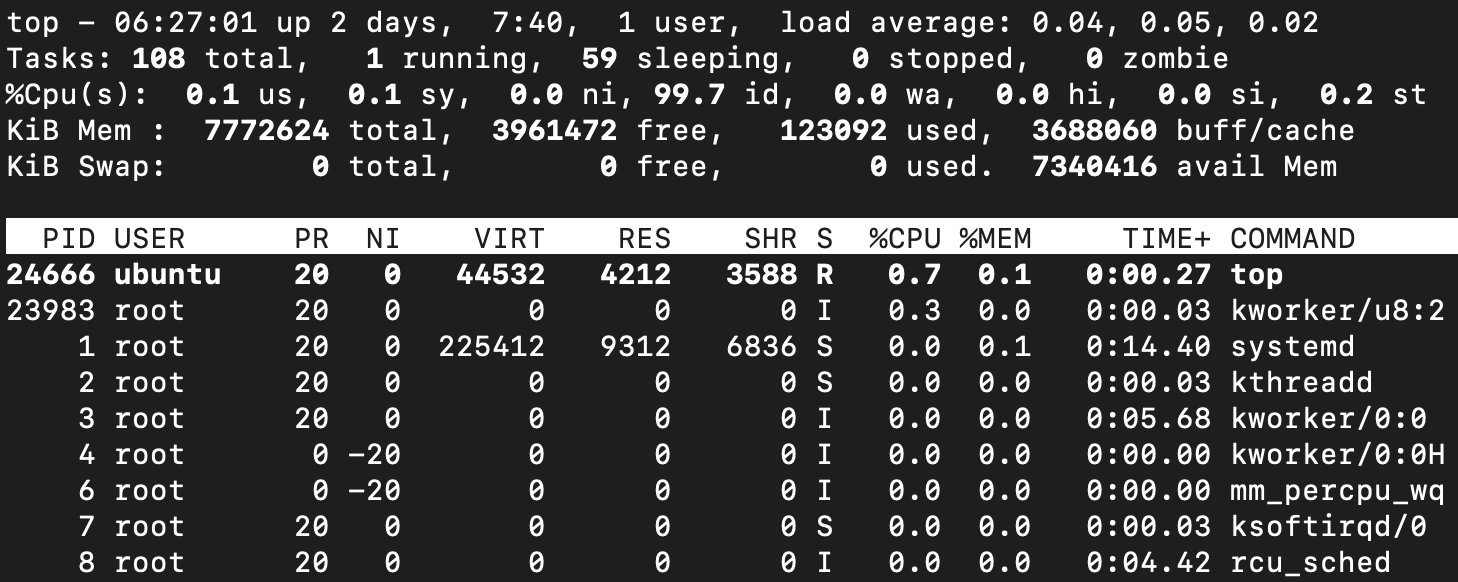
\includegraphics[scale=0.60]{10-2.png}
    \par Shown above: sample \verb|top| output
\end{center}

\npar And as an extra note, \verb|htop| is a more colorful and slightly more informative version of \verb|top|.

\newpage
\section{Checking Disc I/O}

\par \verb|vmstat| is the main linux utility for checking virtual memory statistics. The main columns to look at are BI and BO, which represent blocks in (received) and blocks out, respectively.

\begin{center}
    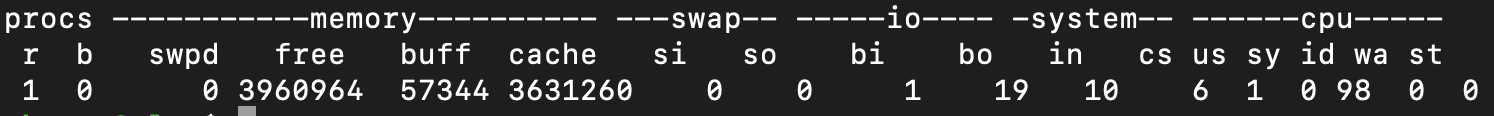
\includegraphics[scale=0.60]{10-3.png}
    \par Shown above: sample \verb|vmstat| output
\end{center}

\section{Approach to Improving Performance}

\par Usually the first thing to look at is your artificial bottlenecks: if your software is poorly written, no amount of sharding and replication will save your application.

\vpar Afterwards, we can move onto checking logs and using \verb|top|. It is highly recommended to gather all your statistics and logs in one place for better analytics (see Section 8.2/12.1 or Chapter 13).

\vpar Once the bottleneck is found, the things to do are (in a rough order): check your app's configurations, review code (if applicable), and scale up (easier thing to do) or scale out.

\vpar In practice we care a lot about our \textbf{tail latencies}, that is, the higher percentiles. There's always going to be something that is slow, but we want to reduce the worst-case times for users.

\chapter{Machine Learning}

\section{Why use it?}

\par We use machine learning (ML) because we are incapable of coming up with an algorithm for the problem. The most popular uses for ML are: computer vision (CV), natural language processing (NLP), and recommendation systems.

\section{ML Types and Models}

\subsection{Supervised vs. Unsupervised}

\par \textbf{Supervised learning} is where the model is fed output that is labelled with the correct answers. An example is a training model where objects in an image are already tagged -- the machine then learns the characteristics of the tagged objects and can identify future objects using their characteristics. Common uses for supervised learning are classification (more later) and regression (prediction and forecasting).

\vpar \textbf{Unsupervised learning} is the exact opposite: none of the outputs are labeled, and the machine must act on the information without guidance. An example is a model that is trained on images of oak and willow trees -- the model can categorize the two based on their characteristics and differentiate them. Common uses for unsupervised learning are clustering (finding groupings in the data) and association (finding rules that describe data, e.g., people who play X tend to play Y).

\subsection{Neural Networks}

\par \textbf{Neural networks} are a general classification for all machine learning algorithms where input data is sent to a "neuron" that does a dot product of the data with weights (which then forwards it to neurons of the next layer, ..., until we reach the output). \textbf{Artificial neural network} is the more official term, differentiating the ML side from an actual biological neural network (our brains).

\vpar In the case of a \textbf{convolutional neural network} (CNN), each weight is represented by a matrix, which is then used to produce a pixel. Specifically, CNNs slide a kernel across dimensions to produce an image. We use an image to explain CNNs because it is most commonly applied to visual imagery. We use this method because in a way it allows the model to also pick up on the surroundings of an image as well.

\vpar \textbf{Long short-term memory (LSTM)} is a neural network that introduces a memory unit called the \textbf{cell}, which stores data useful for computations across all units (which may alter the memory). A popular use of an LSTM is in \textbf{transformers}, which translates one sequence to another. An example of a transformer is for language translation -- using an LSTM, the neural net is able to use past words to give context to future ones.

\newpage
\subsection{Classification, Detection, Segmentation}

\par All techniques listed above fall under computer vision, which we describe below:

\begin{itemize}
    \item \textbf{Classification}: labelling what is in the video (doesn't say where it is, just if it exists)
    \item \textbf{Detection}: distinguishing distinct objects in an image/video, separating them using bounding boxes
    \item \textbf{Segmentation}: providing an exact outline of each object that is classified
\end{itemize}

\section{ML Techniques}

\subsection{Embedding}

\par \textbf{Embedding} is the process of projecting an input into a better representation space. In this class, we specifically refer to the transformation of words into numbers for easier processing.

\section{Miscellaneous Terms}

\begin{itemize}
    \item \textbf{Overfitting}: Training a model too closely to a particular set of data, such that it is unable to generalize and is unable to fit additional data points.
    \item \textbf{Hidden Layer}: Essentially any layer in an artificial neural network that isn't the input or output (anything in between). It takes the weighted inputs and produces output using an activation function. 
\end{itemize}

\chapter{Monitoring and Security}

\section{Introduction to Monitoring}

\par Outside of \verb|top|, the most popular (and scalable) method of discovering bottlenecks, bugs, and any issues is to use a monitoring service. Most monitoring services are \textbf{agent-based}, where agents report metrics to a main server, which aggregates all the data. 

\note Generally, an agent is usually software that runs in the background for \textit{another user or program}, which differentiates it from a daemon.

\section{Security Practices}

\par Here we talk about best practices for security:

\subsection{Password Hashing}

\par \textbf{Password hashing} is the act of performing a one-way transformation on a password, such that it is impossible to turn the hashed password back to its original. That way, if a collection of password were somehow compromised, hackers still wouldn't be able to log into the system since they can't reverse it.

\section{Security Vulnerabilities}

\par In this section, we talk about various vulnerabilities possible in any system:

\subsection{Server-side Code Injection}

\par In a \textbf{server-side injection attack}, the attacker submits malicious input which gets executed on the server. The input could be submitted in various ways, such as web forms or URL parameters.

\vpar One of the prerequisites for a server-side attack is to gain an understanding of the back-end application -- a common method is to use an information disclosure attack, but we won't go into that here.

\vpar Some examples of a server-side attack: SQL injection, command injection (like shell?), and buffer overflow attacks.

\newpage
\subsection{Client-side/Cross-site Code Injection}

\par \textbf{Cross-site (XSS) injections} work similarly to server-side ones; instead of SQL or shell commands, script tags are entered into web forms (or anything that allows info to be saved into the DB). Once the script tags are in the database, any user who queries that script tag will run malicious code which can send private data to the attacker's private server (or worse). This kind of attack is usually referred to as a \textit{stored} XSS attack.

\vpar Another kind of XSS is a \textit{reflected} attack, here the attacker sends a malicious link/URL to a user, which contains a script tag in its query parameters. This attack usually involves more social engineering or mass-sending of emails to work, as well as a lack of data escaping of the insecure website which allows script tags as query parameters.

\chapter{Analytics}

\section{MapReduce}

\par \textbf{MapReduce} is a processing technique/algorithm for processing/generating huge datasets on a cluster. The procedure is composed of 3 parts:

\begin{enumerate}
    \item Map: Performs the conversion of data -- more specifically, it takes key/value pairs and produces another set of intermediate key/value pairs
    \item Shuffle: Said to be part of the Reduce phase, shuffling is where intermediate data from mappers are transferred to reducers
    \item Reduce: Performs a summary operation to create a smaller set of tuples (producing zero or more outputs)
\end{enumerate}

\section{Apache Hadoop}

\par \textbf{Apache Hadoop} is a collection of open-source software utilities (library) that allows for distributed processing of large datasets across clusters of computers. Its main strengths is its ability to work efficiently on parallel and on cheap hardware. It is comprised of 4 main modules:

\begin{itemize}
    \item Hadoop Common: libraries and modules used by all other Hadoop modules
    \item HDFS: distributed file-system that stores data, providing high bandwidth
    \item Hadoop YARN: platform responsible for managing computing resources in clusters and using data to schedule applications
    \item Hadoop MapReduce: implementation of MapReduce programming model for large-scale data processing
\end{itemize}

\npar Hadoop is good for long-running batch jobs -- however, for real-time use, not so much.

\section{Apache Spark}

\par \textbf{Apache Spark} is another popular distributed computing framework. Spark is better for real-time processing, but is highly dependent on doing stuff from memory -- reading stuff from disk is going to kill it. Its more likely to be seen in a smaller startup, maybe with less data.

\end{document}
